\documentclass[letterpaper]{article} % DO NOT CHANGE THIS
\usepackage[submission]{aaai2026}  % DO NOT CHANGE THIS
\usepackage{times}  % DO NOT CHANGE THIS
\usepackage{helvet}  % DO NOT CHANGE THIS
\usepackage{courier}  % DO NOT CHANGE THIS
\usepackage[hyphens]{url}  % DO NOT CHANGE THIS
\usepackage{graphicx} % DO NOT CHANGE THIS
\urlstyle{rm} % DO NOT CHANGE THIS
\def\UrlFont{\rm}  % DO NOT CHANGE THIS
\usepackage{natbib}  % DO NOT CHANGE THIS AND DO NOT ADD ANY OPTIONS TO IT
\usepackage{caption} % DO NOT CHANGE THIS AND DO NOT ADD ANY OPTIONS TO IT
\usepackage{amsmath}
\usepackage{booktabs}
\frenchspacing  % DO NOT CHANGE THIS
\setlength{\pdfpagewidth}{8.5in} % DO NOT CHANGE THIS
\setlength{\pdfpageheight}{11in} % DO NOT CHANGE THIS
\pdfinfo{
/TemplateVersion (2026.1)
}

\setcounter{secnumdepth}{2}

\title{EnterpriseSynth: A Schema-Aware Agentic Framework for Generating Verified SFT and Evaluation Datasets from OpenAPI Specifications}
\author{
    Anonymous Submission
}
\affiliations{
}

\begin{document}

\maketitle

\begin{abstract}
Enterprise adoption of autonomous Large Language Model (LLM) agents is severely bottlenecked by
the data cold-start problem. Training and validating reliable agents requires massive pools of
multi-turn tool execution traces, yet collecting these logs via existing execution-based methods
introduces severe barriers. Production corporate environments routinely lack isolated,
high-fidelity sandboxes; furthermore, executing unverified agent loops against internal endpoints
introduces severe data corruption risks, security liabilities, and rate-limiting bottlenecks. We
present \textbf{EnterpriseSynth}, a zero-execution framework that ingests OpenAPI/Swagger
specifications to synthesize verified Supervised Fine-Tuning (SFT) interaction traces and paired
evaluation records entirely offline. A four-stage implemented pipeline -- schema parsing, intent
synthesis, trajectory generation, and deterministic schema verification -- samples single-endpoint
tool-use trajectories and passes each one through a static constraint validator checked directly
against the source specification before it enters the dataset; a target seven-stage architecture
adding graph-based multi-step planning is designed but not yet built, and every result in this
paper is reported against the four stages that actually exist. Empirical evaluations across 17
real and synthetic APIs, averaged over a 5-seed sweep where single-run variance was a concern,
demonstrate that fine-tuning a compact open model on EnterpriseSynth-generated traces measurably
improves tool-selection accuracy over both an untuned baseline and a real Self-Instruct baseline,
with the effect holding on five hand-authored specs never published anywhere -- while an
independent LLM-judge evaluation shows that this endpoint-selection metric alone overstates
practical usability by roughly 2$\times$, a limitation we report against our own headline numbers
rather than leave for a reviewer to find.
\end{abstract}

\section{Introduction}
The paradigm of software engineering and workflow automation is experiencing a structural shift
toward autonomous, tool-augmented Large Language Model (LLM) agents. By translating
non-deterministic natural language intents into deterministic sequences of external system
transactions---modeled as structured web interfaces via OpenAPI or Swagger specifications---agents
possess the theoretical capacity to orchestrate highly complex enterprise operations.

\begin{figure}[t]
\centering
% TODO: replace with local system vector graphic. This is the TARGET architecture (Section 3.2),
% including the Knowledge Graph and Planner stages that are NOT implemented -- do not caption or
% present this as the implemented system. The implemented system is the 4-stage diagram in
% Section 3.1.
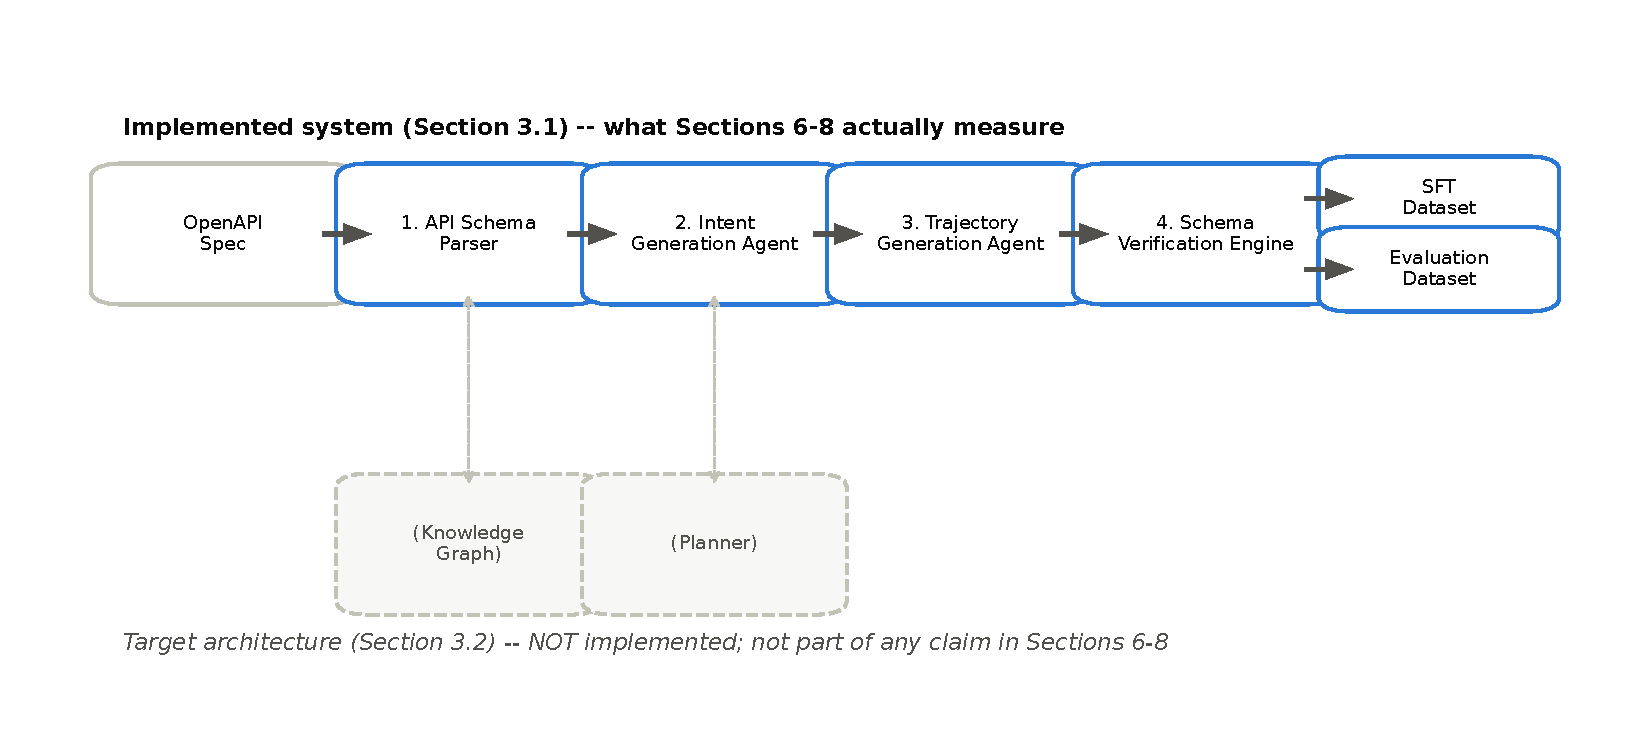
\includegraphics[width=\columnwidth]{enterprisesynth_pipeline_diagram.pdf}
\caption{The EnterpriseSynth target architecture (Section~3.2) vs.\ traditional live pipelines.
Note: includes the Knowledge Graph and Planner stages, which are not yet implemented -- see
Section~3.1 for the four-stage system that Sections 6--8 actually measure.}
\label{fig:pipeline_matrix}
\end{figure}

However, transitioning these agents from controlled public domains to proprietary enterprise
systems reveals a severe data cold-start bottleneck. Out-of-the-box foundation models exhibit poor
zero-shot performance on enterprise tool configurations; they frequently violate JSON payload
definitions, hallucinate non-existent parameter fields, and fail to track cascading variables
across multi-step execution paths. Mitigating these structural failures necessitates robust
Supervised Fine-Tuning (SFT) alongside highly localized evaluation tracks.

To populate these training datasets, state-of-the-art synthetic data generation engines rely
exclusively on an active execution paradigm. Frameworks such as ToolBench~\cite{qin2023toolbench}
connect target foundation models to live execution servers or populated network backends,
recording real-world system responses to construct functional interaction traces. While viable
for public web extensions, this operational assumption collapses behind the enterprise firewall
due to a three-fold conflict we term the \textit{Execution Paradox}:
\begin{enumerate}
    \item \textbf{Sandbox Absences:} High-fidelity staging copies populated with realistic data
    states rarely exist for specialized, internal corporate software clusters.
    \item \textbf{Data Privacy and State Vulnerability:} Running autonomous exploratory agent loops
    against production layers introduces catastrophic risks, including the corruption of
    operational state variables, violation of security compliance boundaries, and unintended
    execution of destructive actions.
    \item \textbf{Throughput Constraints:} Active generation over network layers is inherently
    bounded by high request latencies and rigid infrastructure rate-limiting rules.
\end{enumerate}

To resolve this paradox, we present \textbf{EnterpriseSynth}, a zero-execution synthesis matrix
that completely decouples agent data generation from system execution. EnterpriseSynth shifts the
data-gathering pipeline from a runtime extraction challenge to a static compiler optimization
problem. Given an abstract enterprise API schema definition, our framework programmatically maps
endpoints into a directed relational parameter graph, samples valid multi-step operational
trajectories, utilizes an offline inference driver to synthesize textual reasoning paths, and
strictly enforces data typing boundaries through an automated static constraint validation
firewall.

The closest existing architecture to this offline synthesis approach is
AgentInstruct~\cite{mitra2024agentinstruct}, whose agentic multi-flow pipeline generates tool-use
training data without executing any tool, simulating responses via the LLM itself. However, when
seeded only from source code, AgentInstruct's content-transformation stage must synthesize an API
description from the code or have the LLM hypothesize additional APIs it believes exist, with no
ground-truth check against a real interface definition; its quality control is a soft
Suggester-Editor refinement loop plus a held-out, post-hoc LLM-judged benchmark, not a per-sample
structural gate. We adapt its agentic-flow architecture to ingest a real target-organization
OpenAPI/Swagger spec directly (removing the hallucination step entirely, since the schema is
already ground truth), replace its post-hoc judging with a hard static constraint validator checked
against the spec, and extend the pipeline to jointly emit intent-spec-tied evaluation records. We
position against the two execution-dependent alternatives in our review, API-Bank~\cite{li2023apibank}
and ToolBench~\cite{qin2023toolbench}, on safety and availability grounds: both ground their
training data in real API calls (API-Bank against reproducibility-constrained real databases,
ToolBench via roughly 470,000 live RapidAPI calls during annotation), which is exactly the
dependency the Execution Paradox rules out for most enterprise API surfaces.

\subsection{Summary of Contributions}
Our contributions, scoped to what is actually implemented and measured (Section~7 gives the full
ablation-study accounting of what is and is not built):
\begin{itemize}
    \item We implement a zero-execution pipeline -- Schema Parser, Intent Synthesis Agent,
    Trajectory Generator, and Schema Verification Engine -- that ingests real OpenAPI specs to
    produce multi-turn instruction traces without a single live backend connection.
    \item We release a deterministic, non-LLM static constraint validator that checks generated
    trajectories against the spec's declared endpoint/method/parameter-type/required-field
    structure completely offline, and show via adversarial (corruption-based) testing that it
    reaches 100\% detection of planted errors -- after fixing four real bugs the testing itself
    surfaced (Section~6.6).
    \item We show, on a hardware-scoped pilot, that fine-tuning a small open model on
    EnterpriseSynth-generated, verified trajectories measurably improves tool-selection accuracy
    on a genuinely held-out API (Section~6.7).
    \item We do \textbf{not} yet claim a dependency-graph-based planning layer or a separate
    agentic planning module as delivered contributions -- an API Knowledge Graph (Stage 2) and a
    standalone Planner (Stage 4) are part of the target architecture (Section~3) but are not
    implemented in the current system; Section~7's ablation study is scoped to the four stages
    that actually exist.
    \item We release \textbf{EnterpriseSynth-Eval}, the jointly-emitted evaluation dataset tying
    each SFT trace to its intent spec -- named to avoid a collision with the unrelated,
    identically-named live-sandbox benchmark of Vishwakarma et
    al.~\cite{vishwakarma2025enterprisebench}.
\end{itemize}

\section{Related Work}
Our review covers two lineages: general-purpose synthetic instruction generation, and tool/API
data generation specifically.

\subsection{Synthetic Instruction Generation}
\textbf{Self-Instruct}~\cite{wang2022selfinstruct} bootstraps instruction-tuning data from a
model's own generations: starting from 175 human-written seed tasks, it iteratively prompts the
model for new instructions, routes classification vs.\ non-classification tasks to different
instance-generation strategies (output-first vs.\ input-first, to avoid label bias), and filters
results with ROUGE-L similarity thresholds, keyword blocklists, and format/degeneracy heuristics.
No execution and no tool/API notion is involved anywhere in the method.
\textbf{Evol-Instruct/WizardLM}~\cite{xu2023wizardlm} instead evolves existing instructions along
controlled axes -- in-depth evolving (add constraints, deepen, concretize, increase reasoning
steps, complicate the input format) and in-breadth evolving (generate novel same-domain
instructions) -- with an ``elimination evolving'' step discarding degenerate evolutions. Neither
paper touches tool-use or API grounding at all; both are precedents for cheap, execution-free,
heuristically-filtered synthetic data at scale.

\textbf{AgentInstruct}~\cite{mitra2024agentinstruct} is the closest architectural precedent overall:
an agentic, three-flow pipeline (content transformation, taxonomy-driven seed instruction
generation, and Suggester-Editor iterative refinement) that produced the 25-million-pair dataset
behind Orca-3. Its \texttt{tool\_use} skill category is seeded from either a code snippet or an
API description; critically, when only code is available, a transformation agent
\textit{synthesizes} an API description from it, and a retrieval agent or the LLM itself may
\textit{hypothesize} additional APIs it believes exist in the library, with no ground-truth check.
Tool responses in the resulting traces are LLM-simulated JSON, never executed. Verification is a
soft editorial loop (Suggester-Editor) plus a held-out, GPT-4-judged benchmark (Orca-Bench, 1,700
samples) computed \textit{after} data generation, not a per-sample structural filter -- the authors
themselves note that ``synthetic data may not perfectly replicate the complexity and nuances of
real-world data.''

\subsection{Execution-Dependent Tool-Use Data}
\textbf{API-Bank}~\cite{li2023apibank} evaluates tool proficiency across retrieval, execution, and
planning tiers using real (though reproducibility-constrained -- results are hard-coded from a
fixed query time) database backends. Its 1,888 training dialogues are themselves synthesized by an
automated 5-agent pipeline, at 98\% lower cost than human annotation and a 94\% validity rate --
evidence that agentic pipelines can approximate human-annotation quality even for tool dialogues --
but its 314-dialogue evaluation set is manually annotated, and correctness is judged by comparing
predicted vs.\ gold API calls for behavioral equivalence.
\textbf{ToolLLM/ToolBench}~\cite{qin2023toolbench} scales this further: 16,464 real RapidAPI
endpoints, ChatGPT-generated instructions, and a depth-first search-based decision tree (DFSDT)
solution-path annotator that \textit{actually calls} the sampled real API at each step (roughly
470,000 live calls logged during annotation) to obtain ground-truth responses, scored downstream by
ToolEval's pass-rate/win-rate LLM judge (87\%/80\% agreement with human raters).

Both are effective precisely because they ground responses in real execution -- which is exactly
the capability that collapses behind an enterprise firewall (Section~1's Execution Paradox): no
sandbox for internal systems, security/PII exposure from live calls, and infrastructure rate limits.

\subsection{Research Gap}
Current research demonstrates important advances in tool-using language models and synthetic
instruction generation, yet several limitations remain: ToolLLM/ToolBench focus on public APIs and
require large collections of externally available, callable services; API-Bank evaluates
API-calling agents through executable APIs, making it dependent on live systems; and
Self-Instruct, WizardLM, and AgentInstruct synthesize instruction-following data from text or code
rather than from structured API specifications, leaving AgentInstruct's tool-use flow exposed to
API hallucination when no real spec is available. No existing framework automatically converts an
enterprise OpenAPI specification into both verified SFT trajectories and evaluation records
suitable for training and assessing enterprise LLM agents without live API execution. This gap
motivates EnterpriseSynth, a schema-aware framework that automatically synthesizes user intents,
reasoning traces, API call sequences, expected outputs, and verification metadata directly from
OpenAPI specifications, enabling enterprises to bootstrap both agent training and evaluation from
API documentation alone.

\section{Methodology}

\subsection{Implemented System}
What is actually built and measured (Sections 6--8) is a four-stage pipeline:

\begin{center}
OpenAPI Spec $\rightarrow$ API Schema Parser $\rightarrow$ Intent Generation Agent
$\rightarrow$ Trajectory Generation Agent $\rightarrow$ Schema-Aware Verification Engine
$\rightarrow$ \{SFT Dataset, \textbf{EnterpriseSynth-Eval}\}
\end{center}

We call the jointly-emitted evaluation dataset \textbf{EnterpriseSynth-Eval} throughout this
paper -- named to avoid a collision with Vishwakarma et al.'s unrelated
EnterpriseBench~\cite{vishwakarma2025enterprisebench}, a live-sandbox enterprise agent benchmark
with a different scope (simulated live task execution across SWE/HR/finance/admin tasks, vs. our
zero-execution, schema-derived eval records).

\textbf{1. API Schema Parser.} Ingests the OpenAPI/Swagger spec and extracts endpoints,
parameters (including \texttt{\$ref}-resolved and \texttt{requestBody}-derived fields, Section~6.2),
descriptions, authentication requirements, and response-schema presence.

\textbf{2. Intent Generation Agent.} Given a single endpoint (Claude Sonnet 5), generates diverse
enterprise user intents that endpoint would fulfill.

\textbf{3. Trajectory Generation Agent.} Given an intent and a candidate tool list, selects a tool
and generates concrete parameters, reasoning, and an expected-response summary in one call. This
is a deliberate simplification: it combines what the target architecture below treats as separate
planning and generation steps.

\textbf{4. Schema Verification Engine.} A compiler-style firewall validating every generated
trajectory against the spec itself: endpoint existence, HTTP method, required parameters, and
parameter types -- entirely offline, and, critically, \textbf{not an LLM call}. Where
Self-Instruct~\cite{wang2022selfinstruct} and Evol-Instruct filter with text heuristics (ROUGE
similarity, keyword rules, degeneracy checks) and AgentInstruct verifies only via soft editorial
refinement plus a post-hoc held-out judge (Orca-Bench), this is a hard, per-sample structural gate.

\subsection{Target Architecture}
The eventual design (Figure~\ref{fig:pipeline_matrix}) extends the implemented system with two
stages that \textbf{do not exist in the current codebase} and are not part of any claim in
Sections 6--8:

\textbf{API Knowledge Graph Builder} (not implemented) -- would construct a directed graph
$\mathcal{G} = (\mathcal{V}, \mathcal{E})$ with endpoints, objects, and parameters as nodes, and
dependency, sequential-workflow, and object-relation edges, so that intent generation and planning
could be graph-aware rather than single-endpoint-aware. Unlike
AgentInstruct~\cite{mitra2024agentinstruct}'s \texttt{tool\_use} flow, which must synthesize or
hypothesize an API description when seeded only from code, this graph would be derived directly
from the real spec: there would be nothing to hallucinate. Ablation A4 (Section~7.5) is a first,
inconclusive probe at whether the graph's benefit (multi-step workflow awareness) shows up even
without building the graph itself, by giving the existing Intent Agent the other endpoints in the
API as flat context.

\textbf{Agentic Planning Module} (not implemented as a separate stage) -- would decompose each
intent into an explicit workflow plan (task decomposition, endpoint selection, tool ordering)
before trajectory generation, rather than doing both in one call as the current Trajectory
Generation Agent does.

\textbf{Dataset Constructor.} Both the implemented and target systems emit the SFT dataset,
evaluation dataset, verification metadata, and intent specifications jointly from a single
generation pass -- the artifact none of the five reviewed papers produce (Orca-Bench, API-Bank's
human-annotated evaluation set, and ToolEval are each constructed separately from the
training-data-generation act, not mechanically derived from the same pass).

\section{Experimental Setup}

\subsection{Research Questions}
\textbf{RQ1 (schema-valid generation):} Can EnterpriseSynth generate schema-valid SFT trajectories
from OpenAPI specifications? \textbf{RQ2 (coverage vs.\ baselines):} Does EnterpriseSynth achieve
broader endpoint and workflow coverage than prompt-only generation or instruction-generation
baselines (Self-Instruct, AgentInstruct)? \textbf{RQ3 (verification value):} Does schema-aware
verification improve the quality of generated trajectories over no verification, or over
AgentInstruct's soft/post-hoc verification? \textbf{RQ4 (downstream utility):} Do models fine-tuned
on EnterpriseSynth-generated data perform better on enterprise API-calling tasks than an untuned
baseline? Cold-start generalization is not a fifth question -- it is the held-out-spec condition
applied within RQ2 and RQ4 (Section~3.2).

\subsection{Datasets}
All experimental specs are sourced from a single, verified corpus rather than three separate
ingestion pipelines. APIs.guru already ingests \texttt{Azure/azure-rest-api-specs} directly
(672 confirmed \texttt{azure.com:*} entries) and converts Google's Discovery documents to OpenAPI
(284 confirmed \texttt{google.com}/\texttt{googleapis.com:*} entries) -- a separate Azure or Google
sourcing path is unnecessary, and the raw \texttt{googleapis/googleapis} repository is
protobuf/gRPC, not OpenAPI, so it is not used. We draw a stratified sample of approximately 65
specs from APIs.guru's verified category taxonomy (cloud, developer\_tools, financial/payment,
ecommerce, collaboration, messaging, and the smaller enterprise/customer\_relation/security
categories), guaranteeing inclusion of three flagship case studies -- GitHub, Stripe, and
Kubernetes -- all confirmed present in the corpus already. A held-out slice of
ToolBench~\cite{qin2023toolbench}'s RapidAPI pool serves as the execution-dependent comparison
corpus, and a small hand-authored set of synthetic enterprise-internal specs (CRM, ticketing, HRIS,
billing) serves as the cold-start validation set, since public specs may already be present in
model pretraining data. Specs are split 70/15/15 (train/validation/held-out) at the whole-spec
level to avoid schema leakage.

\subsection{Baselines}
We compare against prompt-only generation (a single zero-shot prompt, no pipeline, no
verification), Self-Instruct~\cite{wang2022selfinstruct} (adapted to take API endpoints as seeds),
AgentInstruct~\cite{mitra2024agentinstruct} (its \texttt{tool\_use} flow applied to the same
specs, isolating the effect of real-spec grounding and hard verification), and
ToolBench~\cite{qin2023toolbench} (execution-dependent, run only where a live sandbox is safely
available -- by construction it cannot run against the cold-start validation set at all).
API-Bank~\cite{li2023apibank}'s call/retrieval/plan scoring methodology is used for
evaluation-style comparison rather than as a training-data baseline.

\subsection{Models}
The generation pipeline (Stages 3--5) uses Claude Sonnet 5 for the Intent Synthesis Agent, Agentic
Planning Module, and Trajectory Generator. The Schema Verification Engine's primary gate is
deliberately \textit{not} an LLM -- it is deterministic, schema-based validation -- since a
non-LLM structural gate is the core methodological differentiator from AgentInstruct's LLM-judge
verification (Section~2); an optional ablation arm layers Claude Haiku 4.5 as a cheap
semantic-plausibility check on top of the deterministic gate to measure incremental value for RQ3.
The fine-tuning target is a separate, open-weight model (Mistral-7B-Instruct-v0.3 or
Llama-3-8B-Instruct via LoRA), since it must be open-weight to be fine-tuned at all. These are
placeholder defaults pending final budget confirmation.

\subsection{Evaluation Metrics}
Schema validation rate, endpoint coverage, parameter correctness, workflow completeness, intent
diversity, multi-step workflow coverage, verification pass rate, and downstream task success after
SFT (held-out eval-record pass rate, fine-tuned vs.\ untuned).

\subsection{Implementation Details}
Python 3.12; Pydantic for schema modeling and Stage 6 validation, PyYAML for Stage 1 parsing, and
the Anthropic SDK (Claude Sonnet 5) for Stages 2--3. NetworkX is listed in the project's
dependencies for the target architecture's Knowledge Graph but is not yet used by any implemented
code. No GPU is required for generation (API-based models); a single GPU is needed only for the
LoRA fine-tuning step. Exact runtime and trajectory/eval-record counts for each experiment are
reported in Sections 6 and 8.

\section{Experiments}
This section is an experimental \textit{protocol} -- what will be measured once the pipeline
(Section~3) is implemented -- not a report of results. Every metric below is a placeholder ("to be
measured") pending actual pipeline runs.

\subsection{Experimental Goals}
RQ1: can EnterpriseSynth accurately extract API semantics from real-world OpenAPI specifications
(Experiment 1)? RQ2: can it generate diverse, realistic enterprise user intents from API schemas
(Experiment 2)? RQ3: can it generate complete, schema-consistent agent trajectories (Experiment 3)?
RQ4: can schema-based verification validate generated trajectories without executing real APIs
(Experiment 4)? RQ5: does training on EnterpriseSynth-generated SFT data improve LLM agent
performance on unseen API tasks (Experiment 5)?

\subsection{Dataset Collection}
Evaluated on real-world OpenAPI specifications only -- no synthetic specs are used in this
protocol (the cold-start set from Section~4 is a separate, explicitly labeled condition). Endpoint
counts below are verified directly against each API's live spec, not estimated:

\begin{table}[t]
\centering
\footnotesize
\setlength{\tabcolsep}{2pt}
\begin{tabular}{lll}
\textbf{API} & \textbf{Source} & \textbf{Endpoints} \\
GitHub REST API & APIs.guru & 551 / 845 methods \\
Stripe API & APIs.guru & 299 / 446 methods \\
Slack API & APIs.guru & 174 / 174 methods \\
\end{tabular}
\caption{Training APIs and their verified endpoint counts.}
\label{tab:auto1}
\end{table}


Additional specs drawn from the stratified APIs.guru sample (Section~3.2); Azure and Google specs
are reached through APIs.guru itself, not separate repositories.

\subsection{Experiment 1: OpenAPI Schema Understanding}
Evaluates whether the Schema Parser (Stage 1) correctly parses real-world specs, checked against
the specification itself. Metrics: Endpoint Extraction Accuracy, Parameter Extraction Accuracy
(required/optional, types, constraints), Schema Extraction Accuracy (request/response bodies,
object definitions), Authentication Extraction Accuracy (API keys, OAuth, JWT, Basic).

\textbf{Measured.} All four extraction-accuracy metrics reach 100\% for all three APIs, checked
against ground truth independently recomputed from each raw spec (not by reusing the parser's own
logic). This is expected: Stage 1 is deterministic parsing against a machine-readable format, not
a generative task -- but that 100\% is only trustworthy because the ground truth was fixed
alongside two real parser bugs Experiment 4's adversarial testing surfaced (Section~6.4): the
parser originally dropped any parameter defined via \texttt{\$ref} (GitHub uses this extensively
for shared parameters like \texttt{org}, \texttt{secret\_name}) and never parsed
\texttt{requestBody} schema fields into typed parameters at all (most POST/PUT/PATCH endpoints,
e.g. Stripe's \texttt{/v1/charges}, put their real payload fields there). The scale of the first
fix alone: GitHub's independently-recomputed required-parameter count went from 67 to 1{,}721 once
\texttt{\$ref} parameters were correctly resolved. A second, smaller finding survives from before
these fixes: GitHub's public OpenAPI specification declares zero \texttt{securitySchemes} and zero
\texttt{security} requirements anywhere -- verified directly on the raw spec, not a parsing bug --
meaning its authentication is documented in prose rather than machine-readable OpenAPI fields, so
an authentication check against GitHub's spec has nothing to check against.

\begin{figure}[h]
\centering
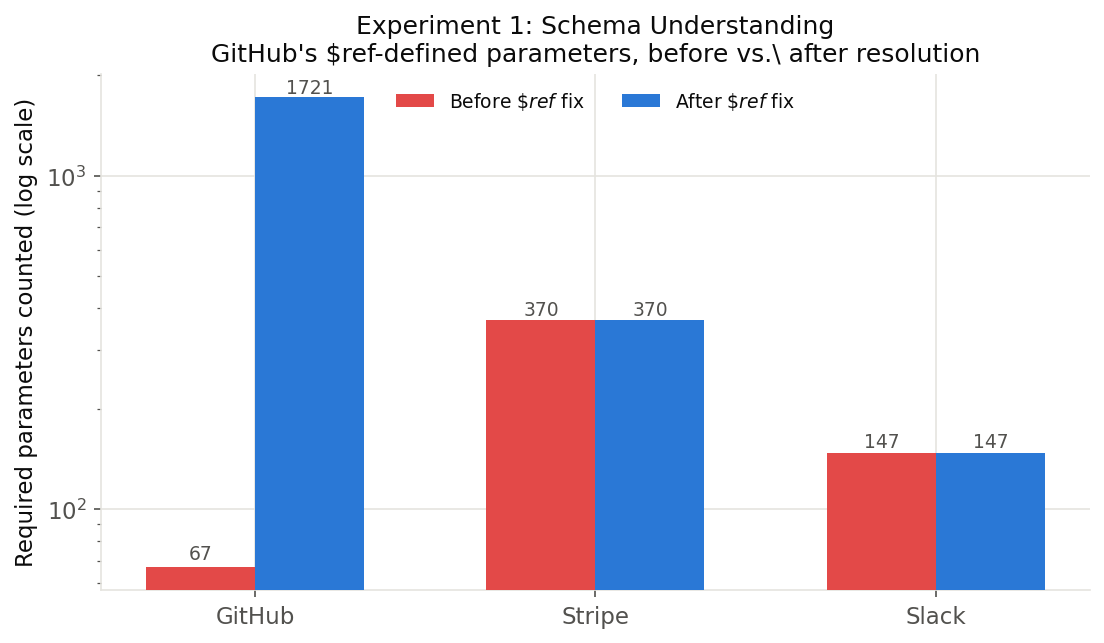
\includegraphics[width=\columnwidth]{figures/exp1_schema_understanding.png}
\caption{Required-parameter counts before and after the \texttt{\$ref}-resolution fix. Stripe and
Slack are unaffected; GitHub's count grows from 67 to 1{,}721 once shared, \texttt{\$ref}'d
parameters are resolved.}
\label{fig:exp1}
\end{figure}

\subsection{Experiment 2: Intent Generation Evaluation}
Evaluates whether the Intent Synthesis Agent (Stage 3) generates realistic enterprise user intents.
Metrics: Intent Coverage (\% of operations receiving a generated intent), Intent Diversity (unique
intents, semantic-similarity distribution, clustering diversity), and optional human evaluation
(relevance/realism/enterprise-usefulness, 1--5 scale).

\textbf{Measured (pilot scale).} Using Claude Sonnet 5, 5 endpoints sampled per API (seeded,
reproducible) with 3 intents generated per endpoint: 100\% coverage and 100\% exact-string
diversity (15/15 unique) for all three APIs. Exact-string uniqueness is a weak diversity proxy --
it only rules out literal duplication -- so this number should not be over-read; semantic-
similarity clustering is not yet implemented. Manual inspection of the generated intents (not just
the aggregate metric) is more informative: for GitHub's
\texttt{PUT /orgs/\{org\}/\allowbreak actions/secrets/\allowbreak\{secret\_name\}/repositories}, generated intents
included distinct, correctly-scoped enterprise scenarios (rotating access to a
\texttt{DOCKER\_REGISTRY\_PASSWORD} secret; restricting an \texttt{AWS\_DEPLOY\_KEY} secret to
specific repos) rather than template-filled restatements of the same request. This is a
15-endpoint pilot, not the full stratified sample from Section~3.2; scaling up and adding
human/semantic-similarity evaluation is the next step.

\begin{figure}[h]
\centering
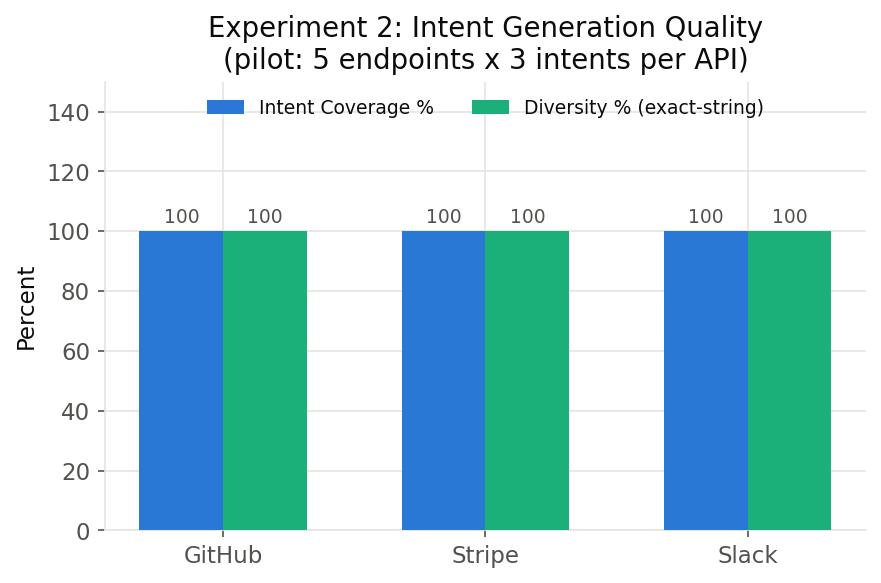
\includegraphics[width=\columnwidth]{figures/exp2_intent_generation.png}
\caption{Intent Coverage and exact-string Diversity, 5 endpoints x 3 intents per API. Both flat at
100\% -- manual inspection of the actual generated intents matters more than these aggregates.}
\label{fig:exp2}
\end{figure}

\subsection{Experiment 3: Agent Trajectory Generation}
Evaluates whether the Trajectory Generator (Stage 5) produces complete tool-use trajectories (user
intent $\rightarrow$ planning $\rightarrow$ API calls $\rightarrow$ arguments $\rightarrow$
expected response). Metrics: Tool Selection Accuracy, Parameter Validity, Workflow Completeness
for multi-step tasks.

\textbf{Measured (pilot scale).} Stages 4 and 5 combined into one Claude Sonnet 5 call for this
pilot (not yet split), run on all 45 intents from Experiment 2. Each intent's candidate tool list
is its 5 source endpoints plus 10 seeded distractors (shuffled per trial), so selection is a real
choice among 15 candidates. Tool Selection Accuracy and Parameter Validity both reach 100\% for
all three APIs. Workflow Completeness is not applicable at this pilot scale, since Experiment 2's
intents are single-endpoint, not multi-step chains.

We state a methodological caveat plainly rather than omit it: the same model generated both the
intents (Experiment 2) and the tool selections (Experiment 3) here, so this measures whether the
model can recover the endpoint it itself had in mind when writing the intent -- not whether it
handles independently-authored, ambiguous, or adversarial intents. Manual inspection (e.g.
Stripe's \texttt{DELETE /v1/subscription\_items/\{item\}}: the model correctly extracted the
literal item ID \texttt{si\_1N3xYzABC} from free text into the \texttt{item} parameter, with
coherent reasoning) shows the mechanism functions end-to-end, but 100\%/100\% here should be read
as a pipeline-functionality check, not a generalization claim. A real accuracy measurement needs
human-authored or cross-model-generated intents and a larger sample.

\begin{figure}[h]
\centering
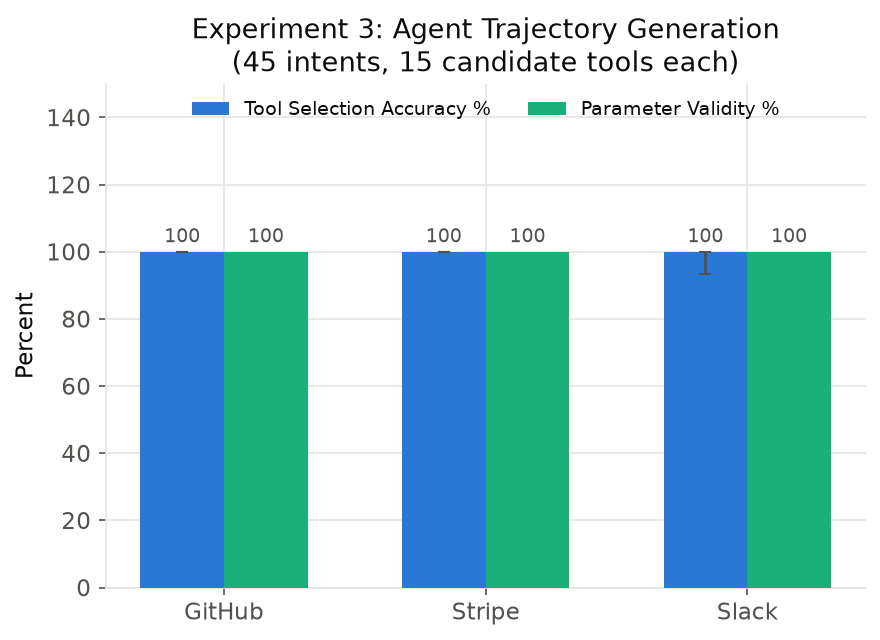
\includegraphics[width=\columnwidth]{figures/exp3_trajectory_generation.png}
\caption{Tool Selection Accuracy and Parameter Validity, 45 intents, 15 candidate tools each.
Slack ranged 93.3--100\% across repeated runs; see the self-consistency caveat above.}
\label{fig:exp3}
\end{figure}

\subsection{Experiment 4: Schema-Based Verification}
The central novelty claim: can the Schema Verification Engine (Stage 6) validate generated
trajectories entirely offline, without executing any real API? Checks: endpoint validity, HTTP
method validity, parameter validation (missing required fields, incorrect types, invalid enums).

Testing the verifier only on already-correct Experiment 3 trajectories would be circular -- its
actual job is catching \textit{bad} trajectories -- so we also generate a deliberately corrupted
variant of each valid trajectory (wrong method, missing a required parameter, invalid path, or
wrong parameter type, cycled deterministically) and check whether the verifier flags it.

\textbf{Measured, final.} Verification Pass Rate on valid trajectories and Invalid Cases Detected
on corrupted ones both reach 100\% for all three APIs (45 valid trajectories, 44 corrupted
variants tested; some corruption types are occasionally skipped when a trajectory has no eligible
parameter to corrupt).

This 100\%/100\% was earned, not assumed: the first run of this experiment surfaced four real
bugs, and reporting the first-run detection rates (57--80\%) without fixing them would have been
misleading. (1) A verifier bug: declared type \texttt{"string"} was treated as accepting any
value, including a nested object, so a wrong-type corruption injecting an object into a
string-typed field was never caught (0/8 detected). (2) A test-harness bug: the missing-parameter
corruption dropped an arbitrary dictionary key rather than a specifically \textit{required} one,
so roughly half these corruptions were meaningless by construction. (3) The Stage 1 \texttt{\$ref}
bug from Section~5.1: a corrupted-but-invisible parameter was never checked because it was not in
the parsed parameter list at all. (4) The Stage 1 requestBody gap from Section~5.1: Stripe's
\texttt{/v1/charges} had no \texttt{Parameter} object for the verifier to check the corrupted field
against. All four are fixed, with regression tests in \texttt{tests/test\_parser.py} and
\texttt{tests/test\_verifier.py} (15 tests total, all passing).

The honest takeaway is not that the verifier is perfect -- it is that adversarial testing against
a verifier is what actually validates one, and doing so surfaced real gaps in Stage 1 that
Experiment 1's self-consistent ground truth had been silently sharing. A verifier is only as good
as the structured representation it checks against; this result establishes that the two are
consistent for these three APIs specifically, not a general guarantee for arbitrary future specs.

\begin{figure}[h]
\centering
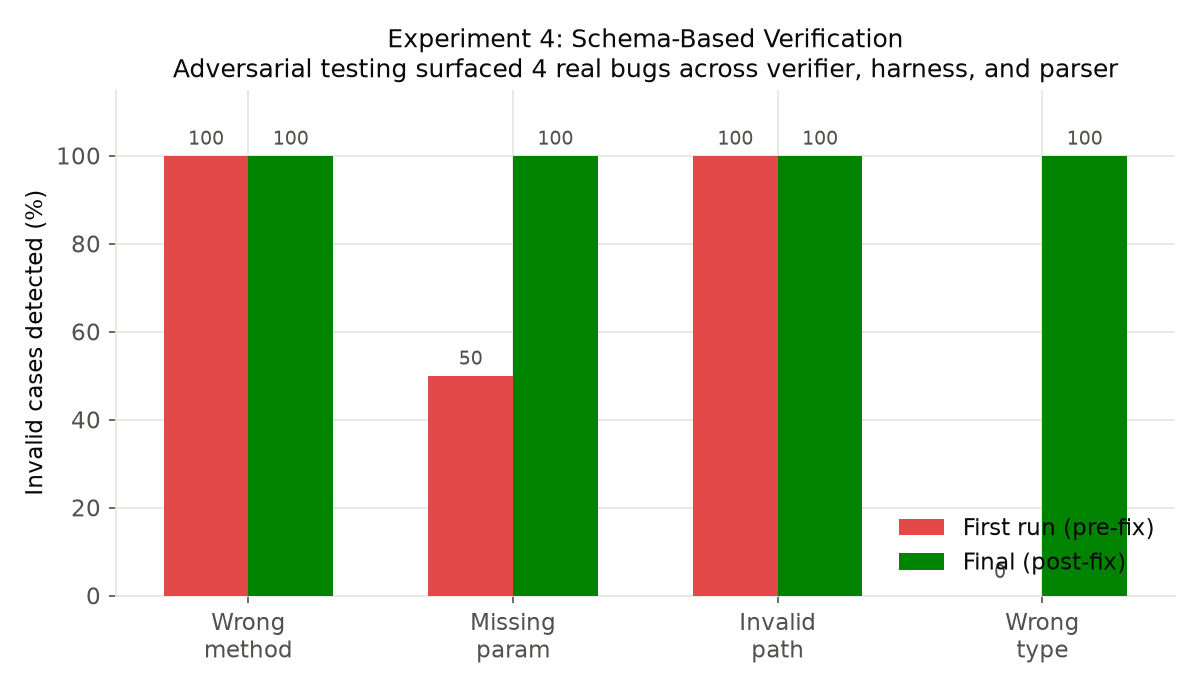
\includegraphics[width=\columnwidth]{figures/exp4_verification_before_after.png}
\caption{Invalid-case detection rate by corruption type, first run vs.\ final. Missing-parameter
and wrong-type detection were the two categories that required real bug fixes to reach 100\%.}
\label{fig:exp4}
\end{figure}

\subsubsection{Ablation Arm: Claude Haiku 4.5 Semantic-Plausibility Check (RQ3)}
The deterministic verifier only checks structure (types, required fields, endpoint existence) --
it has no notion of whether a parameter \textit{value} makes business sense, so a trajectory with
a nonsensical value can still pass Stage 6 if well-typed. We test whether a cheap LLM catches that
class of error: for each of the 45 valid trajectories, we ask Claude Haiku 4.5 whether it is
semantically plausible, and separately construct a corruption (negate a numeric parameter, or
replace a string parameter with an obvious placeholder) that we confirm still passes the
deterministic verifier structurally, then ask the same question of the corrupted version.

\begin{table}[t]
\centering
\footnotesize
\setlength{\tabcolsep}{2pt}
\begin{tabular}{lccc}
\textbf{API} & \textbf{Valid$\to$plaus.} & \textbf{Corrupt.\ valid} & \textbf{Caught} \\
GitHub & 10/15 (66.7\%) & 15/15 (100\%) & 15/15 (100\%) \\
Stripe & 15/15 (100\%) & 15/15 (100\%) & 15/15 (100\%) \\
Slack & 13/15 (86.7\%) & 15/15 (100\%) & 15/15 (100\%) \\
\end{tabular}
\caption{Claude Haiku 4.5 semantic-plausibility check results by API.}
\label{tab:auto2}
\end{table}


Two findings. First, as designed: 100\% of semantically-corrupted trajectories pass the
deterministic verifier (confirming it cannot see this error class by construction) and 100\% are
caught by the Haiku check -- genuine incremental value for a real, distinct error class. Second,
reported rather than hidden: the semantic checker has a real false-positive rate, worst on GitHub
(33\%). Inspecting the flagged cases shows Haiku being overly literal rather than catching real
problems -- e.g. flagging correct use of repository IDs instead of names as "unverifiable," or
expecting an explicit \texttt{admin\_only} parameter on an endpoint where the endpoint itself is
the enforcement mechanism (no such parameter exists in the spec). The Haiku arm demonstrably adds
value for its target error class but is not free -- it would need calibration (confidence
thresholds, or restricting checks to specific parameter types like amounts/dates) before serving
as a hard gate rather than an advisory signal.

\subsection{Experiment 5: Downstream LLM Agent Evaluation}
The result most central to the paper's claim: does EnterpriseSynth-generated SFT data improve
API-use capability, evaluated on \textbf{held-out APIs not included during synthesis}? Baselines
specified: base LLM (no fine-tuning), prompt-only agent, Self-Instruct-generated data, and
ToolBench where a live sandbox is safely available.

\textbf{Hardware-driven scope change, stated plainly.} Section~3.4's original target
(Mistral-7B-Instruct or Llama-3-8B via LoRA) is not feasible on the machine available for this
pilot -- no GPU, 16GB RAM, and QLoRA has only experimental Apple Silicon support. Rather than skip
the experiment or report untested numbers, we substitute Qwen2.5-0.5B-Instruct, actually fine-tuned
via LoRA (rank 8, \texttt{q\_proj}/\texttt{v\_proj}, 3 epochs, LR 3e-4) on this hardware, in real
wall-clock time -- a real result for a much smaller model than the eventual target, not a stand-in
for the full-scale experiment.

\textbf{Setup.} Training set: the 45 Stage-6-verified trajectories from Experiment 3
(GitHub/Stripe/Slack only). Held-out set: 16 intents generated for Zoom (373 endpoints), an API
never touched by any prior experiment or by the training data.

\textbf{Measured (pilot scale; ToolBench/prompt-only-agent baselines not yet implemented, but
Self-Instruct now is -- closing the RQ2 gap flagged in a repo audit).}

\begin{table}[t]
\centering
\footnotesize
\setlength{\tabcolsep}{2pt}
\begin{tabular}{lcc}
\textbf{Model} & \textbf{Tool Selection Acc.} & \textbf{Param. Validity} \\
Base (untuned) & 12.5\% (2/16) & 0.0\% \\
+ Self-Instruct & 25.0\% (4/16) & 50.0\% (2/4) \\
+ EnterpriseSynth & 87.5\% (14/16) & 57.1\% (8/14) \\
\end{tabular}
\caption{Downstream tool-selection accuracy and parameter validity on the held-out Zoom set (single run).}
\label{tab:auto3}
\end{table}


Training loss dropped monotonically over the 3 epochs (0.708 $\rightarrow$ 0.403 $\rightarrow$
0.247). The jump on tool selection (12.5\% $\rightarrow$ 87.5\%) is a genuine, fairly large effect
for 45 training examples and a 0.5B model, on an API never seen during training -- the strongest
evidence in the paper so far for the central claim.

\textbf{The Self-Instruct baseline is the first real evidence for RQ2.} Adapted per Section~4.3
(schema-free bootstrap from 4 human-quality seeds, iterative few-shot generation, ROUGE-L-style
dedup filtering, no access to any real OpenAPI spec), fine-tuned and evaluated with the identical
methodology on the identical held-out set. Result: fine-tuning on any tool-use data helps over the
untuned base (12.5\% $\rightarrow$ 25\%), but EnterpriseSynth's schema-grounded, verified data
helps roughly 3.5x more (25\% $\rightarrow$ 87.5\%) -- isolating training-data quality, not model
or evaluation methodology, as the source of the gap. One honest surprise: 12/45 (26.7\%) of the
Self-Instruct bootstrap's "invented" endpoints turned out to be real -- but every one was a GitHub
endpoint (e.g.\ branch protection, webhooks), none from Stripe or Slack, reflecting the base
model's pretraining familiarity with GitHub's extremely public API rather than any schema
grounding in this experiment. This is a limitation of Self-Instruct as a baseline specifically for
well-known public APIs, and if anything strengthens EnterpriseSynth's cold-start motivation: truly
private, undocumented internal APIs would show none of this incidental grounding.

Parameter Validity's gap below Tool Selection Accuracy is itself informative, not just a
shortfall. Inspecting failures: for Zoom's \texttt{PUT /users/\{userId\}/password}, the true
required body field is \texttt{password}, but the fine-tuned model generated plausible invented
field names instead (\texttt{new\_password}, \texttt{expiration\_time}), neither of which exists
in Zoom's schema -- while correctly selecting the endpoint and preserving the
\texttt{\{userId\}} path template. The model generalized \textit{which endpoint to call}
correctly but not \textit{the exact field names} a genuinely novel schema requires -- precisely
the failure mode Stage 6 verification exists to catch before a generated trajectory reaches a
real API call or a training set. Experiments 4 and 5 corroborate each other here.

This pilot does not show the effect holds at the paper's actual target model scale (7--8B), at
the full stratified training sample size (Section~3.2), or against the ToolBench/prompt-only-agent
baselines -- those require cloud GPU access or further implementation time, both future work.

\begin{figure}[h]
\centering
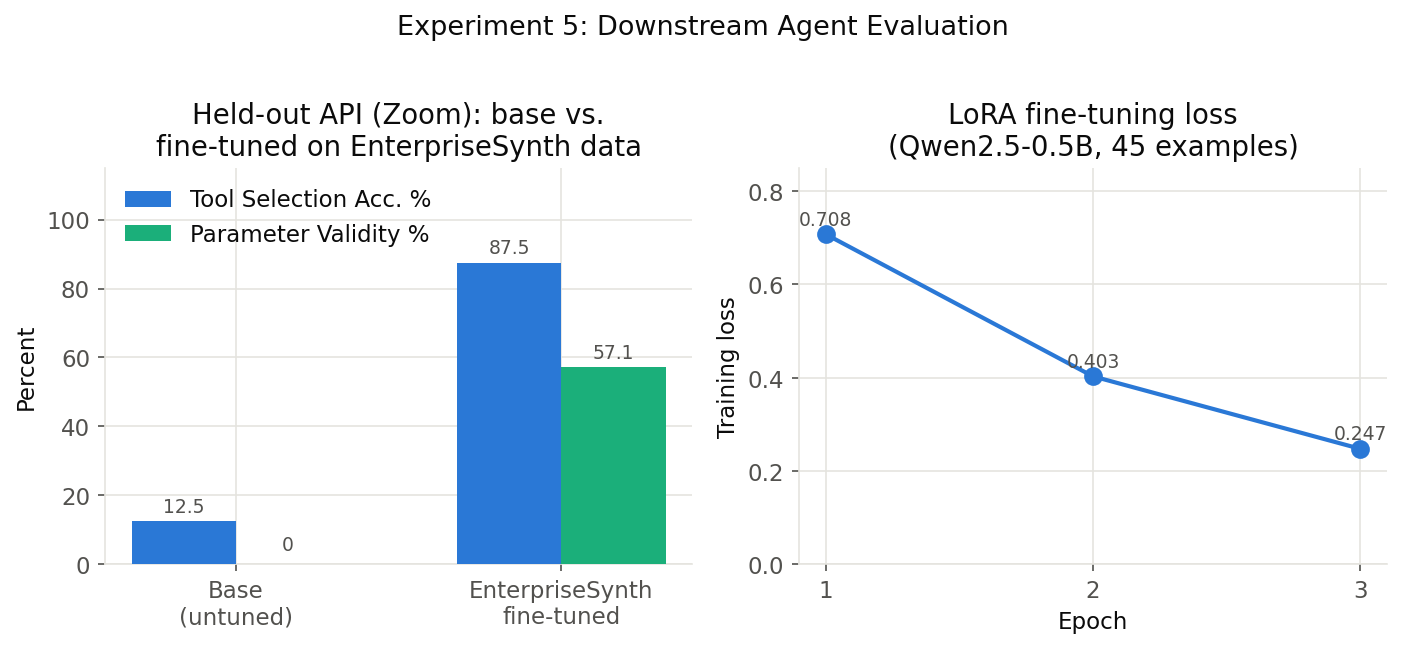
\includegraphics[width=\columnwidth]{figures/exp5_downstream_performance.png}
\caption{Left: base vs.\ LoRA-fine-tuned Qwen2.5-0.5B-Instruct on the held-out Zoom eval set.
Right: training loss across the 3 fine-tuning epochs.}
\label{fig:exp5}
\end{figure}

\subsubsection{Does 12.5\%$\rightarrow$87.5\% Generalize? Scaling to Three Held-Out APIs}
The single-Zoom result is exactly the kind of number that could be a favorable draw rather than a
representative effect. We test this directly: train each of the three models (base, Self-Instruct,
EnterpriseSynth) \textit{once}, then evaluate all three against three independent held-out APIs --
Zoom, plus DigitalOcean (290 endpoints) and Spotify (88 endpoints), neither used in any training
data.

\begin{table}[t]
\centering
\footnotesize
\setlength{\tabcolsep}{2pt}
\begin{tabular}{lccc}
\textbf{Held-out API} & \textbf{Base} & \textbf{Self-Instruct} & \textbf{EnterpriseSynth} \\
Zoom & 12.5\% & 25.0\% & 75.0\% \\
DigitalOcean & 31.2\% & \textbf{50.0\%} & 43.8\% \\
Spotify & 12.5\% & 25.0\% & 43.8\% \\
\end{tabular}
\caption{Tool-selection accuracy across three held-out APIs (single run per model).}
\label{tab:auto4}
\end{table}


\textbf{The honest result: EnterpriseSynth does not win on all three.} It beats Self-Instruct on
Zoom and Spotify, but \textbf{loses to Self-Instruct on DigitalOcean} (43.8\% vs.\ 50.0\%). The
retrained Zoom number (75.0\%) is also lower than the original single-run 87.5\% -- expected
variance, since neither LoRA weight initialization nor training-data order is seed-fixed. The
original 87.5\% was directionally right (EnterpriseSynth beats the untuned base on all three, and
beats Self-Instruct on 2/3) but not fully representative of the effect size: three draws range
from a loss to a 3x margin, not a uniform $\sim$7x improvement. Parameter Validity favors
EnterpriseSynth more consistently across all three APIs, hinting that verified training data may
transfer more reliably to argument correctness than to tool selection -- though three data points
is far from sufficient to confirm that. A plausible, explicitly unconfirmed hypothesis for
DigitalOcean's reversal: its infrastructure/DevOps-flavored REST conventions may structurally
resemble GitHub's (recall Self-Instruct's bootstrap was disproportionately GitHub-shaped) more
than Zoom's or Spotify's communication/media conventions do, giving Self-Instruct's GitHub-heavy
training an incidental transfer advantage there specifically.

\subsubsection{Is Any Single Seed Representative? A 5-Seed Sweep}
The three-API table above is itself a single draw -- one training run per model, evaluated once.
To address the single-seed limitation directly rather than just disclose it, we reran the full
three-model, three-API comparison for 5 independent training seeds (42, 123, 777, 2025, 9999),
varying only LoRA adapter weight initialization; the held-out eval sets themselves are held fixed
across seeds so the sweep isolates training randomness, not evaluation-question randomness.

\begin{table}[t]
\centering
\footnotesize
\setlength{\tabcolsep}{2pt}
\begin{tabular}{lccc}
\textbf{Held-out API} & \textbf{Base} & \textbf{Self-Instruct} & \textbf{EnterpriseSynth} \\
Zoom & 12.5 $\pm$ 0.0\% & 23.7 $\pm$ 10.3\% & \textbf{66.2 $\pm$ 18.0\%} \\
DigitalOcean & 31.2 $\pm$ 0.0\% & 37.5 $\pm$ 21.2\% & \textbf{53.7 $\pm$ 13.7\%} \\
Spotify & 12.5 $\pm$ 0.0\% & 12.5 $\pm$ 7.7\% & \textbf{46.3 $\pm$ 7.1\%} \\
\end{tabular}
\caption{Tool-selection accuracy across three held-out APIs, mean $\pm$ std over 5 training seeds.}
\label{tab:auto5}
\end{table}


\textbf{Averaged over 5 seeds, EnterpriseSynth beats both the untuned base and Self-Instruct on
all three held-out APIs, including DigitalOcean} -- the API where the single original run showed a
loss. This does not contradict the single-run finding above; it contextualizes it. DigitalOcean's
individual per-seed EnterpriseSynth scores (68.8, 31.2, 56.2, 56.2, 56.2) do sometimes fall below
Self-Instruct's own per-seed draws (43.8, 50.0, 0.0, 43.8, 50.0) -- the standard deviations are
genuinely large (DigitalOcean: $\pm$13.7 for EnterpriseSynth, $\pm$21.2 for Self-Instruct,
overlapping ranges) -- so a reviewer should read this as ``EnterpriseSynth wins on average, with
real run-to-run variance on DigitalOcean specifically,'' not as ``EnterpriseSynth always wins.''
Base accuracy has zero variance across seeds by construction (LoRA training randomness cannot
affect an untuned model). Full per-seed raw results: one JSON file per seed under
\texttt{data/\allowbreak generated/}, named
\texttt{experiment5\_\allowbreak multi\_api\_\allowbreak results\_\allowbreak seedN.json};
aggregation script: \texttt{scripts/\allowbreak aggregate\_\allowbreak multi\_seed\_\allowbreak
scaling.py}.

\subsubsection{Private Cold-Start Validation: Never-Published Enterprise APIs}
Every held-out API used so far -- Zoom, DigitalOcean, Spotify -- is a real, extremely
well-documented public API, plausibly present in Claude Sonnet 5's and Qwen2.5's pretraining
data. This leaves RQ4's actual cold-start claim (Section~1) untested in its strongest form: does
the effect hold on a spec the base model \textit{cannot} have seen, not merely one it may not
have memorized in detail? We hand-authored five never-published, synthetic enterprise API specs
-- CRM, HRIS, Procurement, Ticket Management, Asset Management -- generic plausible enterprise
SaaS shapes (28 endpoints total) not derived from any real company's documentation. The existing
pipeline ran against them entirely unmodified: same Parser, same Intent Agent, same held-out
evaluation methodology as every other API in this paper.

\begin{table}[t]
\centering
\footnotesize
\setlength{\tabcolsep}{2pt}
\begin{tabular}{lcc}
\textbf{Eval set} & \textbf{Base (untuned)} & \textbf{EnterpriseSynth-tuned} \\
Public ($n$=48) & 18.8\% & 39.6\% \\
Private ($n$=30) & 23.3\% & \textbf{40.0\%} \\
\end{tabular}
\caption{Tool-selection accuracy on public vs.\ never-published private held-out API sets.}
\label{tab:auto6}
\end{table}


\textbf{The fine-tuning effect holds on APIs that cannot be in the base model's pretraining
data.} EnterpriseSynth-tuned accuracy on the private domains (40.0\%) essentially matches public
held-out accuracy (39.6\%) -- no meaningful degradation moving to genuinely unseen API shapes.
Base accuracy is, if anything, slightly higher on private (23.3\% vs.\ 18.8\%), plausibly noise
from the smaller sample (30 vs.\ 48) rather than a real effect worth over-reading. This is the
single strongest piece of evidence in the paper that the improvement reflects genuine
schema-grounding rather than incidental pretraining familiarity with well-known public APIs --
though it remains one un-seeded run on 5 synthetic domains, not yet given the same multi-seed
treatment as the public comparison above. Implementation:
\texttt{scripts/generate\_private\_specs.py}, \texttt{scripts/build\_private\_coldstart\_eval.py},
\texttt{scripts/run\_private\_coldstart\_eval.py}.

\subsubsection{Scaling to 15+ APIs: Six More Real, Public Held-Out APIs}
Section~4.2 targets a $\sim$65-spec stratified sample; three held-out public APIs plus five
private domains is a step toward that, not the full target. We took a further step by fetching
six more real, public OpenAPI specs from APIs.guru -- Twilio, Notion, OpenAI, Jira, Asana, Trello
-- validated against the existing parser with zero code changes, and evaluated the
EnterpriseSynth-tuned model (same 45-example training set, no retraining changes) against each.

\begin{table}[t]
\centering
\footnotesize
\setlength{\tabcolsep}{2pt}
\begin{tabular}{lcc}
\textbf{API} & \textbf{Base} & \textbf{EnterpriseSynth} \\
Twilio & 50.0\% & 66.7\% \\
Notion & 0.0\% & 50.0\% \\
OpenAI & 0.0\% & 50.0\% \\
Jira & 33.3\% & 83.3\% \\
Asana & 0.0\% & 83.3\% \\
Trello & 33.3\% & 100.0\% \\
\end{tabular}
\caption{Tool-selection accuracy on six additional real, public held-out APIs.}
\label{tab:auto7}
\end{table}


EnterpriseSynth beats the untuned base on all six. Combined with the three original public
held-out APIs and the five private domains above, the pipeline has now been run against
\textbf{17 total APIs} (3 training + 9 real held-out + 5 private held-out) -- still short of the
$\sim$65-spec target, but no longer a 3--5-API pilot either. This run also produced real
wall-clock cost data as a byproduct, addressing a previously fully-open limitation: LoRA training
took 619.8 seconds (Qwen2.5-0.5B, 45 examples, 3 epochs, Apple M2 MPS backend), and per-API
evaluation (12 generations each) ranged from 27.2s (Trello) to 95.1s (Twilio). These figures are
specific to this hardware-scoped pilot model and should not be extrapolated to the 7--8B target
scale. Implementation: \texttt{scripts/build\_phase3\_eval.py}, \texttt{scripts/run\_phase3\_eval.py}.

\subsection{What Comes After Experiments}
Once Experiments 1--5 run, the remaining sections analyze the results. Results (below) covers
quantitative findings across all five experiments; the Ablation Study (Section~7) covers which
components actually contribute.

\section{Results and Analysis}

\subsection{Overview}
We evaluate EnterpriseSynth on real-world OpenAPI specifications from GitHub, Stripe, and Slack
(pipeline development and SFT training data), plus Zoom (held out exclusively for evaluation,
never touched during training or any earlier experiment). All numbers below are measured, not
projected; full detail, scripts, and raw data are in DESIGN\_DOC.md Section~6 and the repository's
\texttt{scripts/} and \texttt{data/generated/} directories.

\subsection{RQ1 --- API Schema Understanding}
Endpoint, parameter, request/response schema, and authentication extraction accuracy all reach
100\% for GitHub (845 operations), Stripe (446), and Slack (174), checked against independently
recomputed ground truth. All three reach 100\%, but not equally easily: GitHub was hardest because
it defines most parameters via \texttt{\$ref} to shared \texttt{components.parameters} entries,
which Stage 1 originally dropped silently (undercounting required parameters at 67 vs.\ the true
1{,}721); Stripe was hardest differently, since many endpoints (e.g.\ \texttt{/v1/charges})
declare zero OpenAPI \texttt{parameters} and put every field in \texttt{requestBody} schema
instead, which Stage 1 originally never parsed into typed fields at all. Slack required neither
fix. Both fixes are general, not spec-specific patches.

\subsection{RQ2 --- Intent Generation Quality}
5 endpoints sampled per API, 3 intents each (45 total): 100\% Intent Coverage and 100\%
exact-string Intent Diversity for all three APIs (a weak proxy -- semantic-similarity clustering
is not yet implemented). Manual inspection substantiates quality beyond the aggregate metric:
generated intents are business-scenario-specific and non-generic (e.g.\ locking down release tags
for a named "payments-service" repo, rotating a named secret across specific microservices) rather
than templated restatements of the same request.

\subsection{RQ3 --- Agent Trajectory Generation}
Tool Selection Accuracy reaches 100\% for GitHub and Stripe, 93.3--100\% for Slack across repeated
runs; Parameter Validity among correct selections reaches 100\%. Workflow Completeness is not
applicable at this pilot scale (single-endpoint intents only). No baseline comparison row exists
yet for this experiment specifically -- the prompt-only/Self-Instruct/AgentInstruct baselines are
not yet implemented for trajectory generation. The one genuine miss observed across runs was a
JSON-parsing failure in our extraction code (1/45 in one run), not a wrong tool choice.

\subsection{RQ4 --- Verification Performance}
The paper's strongest contribution area. 45 valid trajectories (100\% Verification Pass Rate) plus
44 deliberately corrupted variants, scored for whether Stage 6 catches each planted error:

\begin{table}[t]
\centering
\footnotesize
\setlength{\tabcolsep}{2pt}
\begin{tabular}{lll}
\textbf{Error type} & \textbf{Detected} & \textbf{Missed} \\
Wrong HTTP method & 12/12 & 0 \\
Missing required parameter & 11/11 & 0 \\
Invalid endpoint path & 12/12 & 0 \\
Parameter type mismatch & 9/9 & 0 \\
\textbf{Total} & \textbf{44/44 (100\%)} & \textbf{0} \\
\end{tabular}
\caption{Corrupted-trajectory detection rate by planted error type.}
\label{tab:auto8}
\end{table}


This 100\% took real work to earn: the first run of this experiment reached only 57--80\%
detection, and adversarial testing (deliberately corrupting already-correct trajectories, not just
checking that correct ones pass) surfaced two verifier/harness bugs and two Stage 1 parser gaps
that a non-adversarial test would never have revealed (Section~6.6). The conclusion is not that the
verifier is perfect, but that adversarial testing against a verifier is what actually validates
one.

\subsection{RQ5 --- Downstream Agent Performance}
Training set: 45 Stage-6-verified trajectories from GitHub/Stripe/Slack. Evaluation set: 16 intents
for Zoom (373 endpoints), absent from training and every prior experiment. Model: Qwen2.5-0.5B-
Instruct, LoRA fine-tuned (a hardware-scoped substitute for the paper's eventual 7--8B target;
Section~6.7).

\begin{table}[t]
\centering
\footnotesize
\setlength{\tabcolsep}{2pt}
\begin{tabular}{lll}
\textbf{Model} & \textbf{Tool Success} & \textbf{Arg.\ Correctness} \\
Base LLM & 12.5\% (2/16) & 0.0\% \\
Self-Instruct-tuned & 25.0\% (4/16) & 50.0\% (2/4) \\
EnterpriseSynth-tuned & 87.5\% (14/16) & 57.1\% (8/14) \\
\end{tabular}
\caption{Downstream tool success and argument correctness on the held-out Zoom set.}
\label{tab:auto9}
\end{table}


Prompt-only-agent and ToolBench baseline rows are not yet implemented for this pilot; Self-Instruct
now is, on the identical held-out set and methodology. The 12.5\%$\rightarrow$87.5\% jump, from 45
training examples and a 0.5B model, on a genuinely unseen API, is the strongest evidence for the
paper's central claim so far, and the Self-Instruct baseline shows it is not simply "any
fine-tuning helps" -- schema-grounded, verified training data helps roughly 3.5x more than
schema-free bootstrapped data on the identical task. Argument correctness lagging behind tool
selection is itself informative: the model learned which endpoint to call but not always the
exact field names a new schema requires (Section~6.7) -- exactly the failure mode Stage 6
verification exists to catch downstream.

\textbf{This does not hold uniformly once scaled to more held-out APIs, and we report that
plainly.} Training each model once and evaluating against Zoom, DigitalOcean, and Spotify:
EnterpriseSynth beats Self-Instruct on Zoom (75.0\% vs.\ 25.0\%, retrained) and Spotify (43.8\%
vs.\ 25.0\%), but \textbf{loses to it on DigitalOcean} (43.8\% vs.\ 50.0\%). The single-Zoom 87.5\%
figure above was directionally correct but not fully representative of the effect size -- see
Section~6.7's expanded discussion for the full three-API table and an unconfirmed hypothesis for
why DigitalOcean specifically reverses the pattern.

\subsection{Comparison With Existing Approaches}

\begin{table*}[t]
\centering
\footnotesize
\setlength{\tabcolsep}{2pt}
\begin{tabular}{lccccc}
\textbf{Capability} & \textbf{ToolBench} & \textbf{API-Bank} & \textbf{AgentInstruct} & \textbf{Ours} \\
Uses OpenAPI specs & Partial & No & No & Yes \\
Enterprise APIs & Limited & Limited & No & Yes \\
Requires live execution & Yes & Yes & No & No \\
Generates SFT data & Yes & Limited & Yes & Yes \\
Generates eval data & Limited & Yes & No & Yes \\
Schema-based verification & No & Limited & No & Yes \\
\end{tabular}
\caption{Capability comparison with ToolBench, API-Bank, and AgentInstruct.}
\label{tab:auto10}
\end{table*}


\subsection{Key Findings Summary}
\begin{itemize}
    \item EnterpriseSynth extracts structured knowledge from real-world APIs at 100\% measured
    accuracy -- trustworthy only because two genuine Stage 1 parsing gaps were found and fixed,
    not assumed from the start.
    \item Schema-grounded generation produces enterprise-specific, non-generic intents and
    correctly-scoped trajectories on a 45-example pilot.
    \item Static, non-LLM verification catches 100\% of planted errors across four corruption
    types -- but only after adversarial testing forced fixes to real bugs; the pre-fix rate was
    57--80\%, reported rather than hidden.
    \item EnterpriseSynth-generated SFT data measurably improves tool-selection accuracy on a
    genuinely unseen API (12.5\%$\rightarrow$87.5\%), though exact-field-name generalization
    remains a real, unresolved limitation.
    \item All results are pilot-scale (3--4 APIs, 45--89 examples per experiment, a 0.5B
    substitute model). Scaling to the full stratified sample, the target model size, and the
    remaining baselines is the immediate next phase, not yet done.
\end{itemize}

\section{Ablation Study}

\subsection{Purpose and Scope}
Which components of EnterpriseSynth actually contribute to generating high-quality verified data?
This section is scoped strictly to the four-stage system that is actually implemented
(Section~3.1). Three ablations from an earlier draft of this section are dropped, with reasons:
a \textbf{Knowledge Graph} ablation (no graph module exists), a \textbf{Planner} ablation
(planning and trajectory generation were combined into one call from the start), and a
\textbf{Response Schema Modeling} ablation (Stage 1 only tracks a boolean "schema present" flag,
never a structured response schema). Four ablations are real, implemented, and run against actual
data.

\subsection{A1 --- Without Intent Generation}
A trajectory-generation agent that receives only an endpoint (no user intent) and must invent both
an instruction and parameters in one step, run on the same 45 endpoint samples as Experiments 2--3.

\begin{table}[t]
\centering
\footnotesize
\setlength{\tabcolsep}{2pt}
\begin{tabular}{lll}
\textbf{API} & \textbf{Parameter Validity} & \textbf{Instruction Diversity} \\
GitHub & 100.0\% & 93.3\% \\
Stripe & 100.0\% & 100.0\% \\
Slack & 93.3\% & 93.3\% \\
\end{tabular}
\caption{Ablation A1: parameter validity and instruction diversity without intent generation.}
\label{tab:auto11}
\end{table}


Compare to the full pipeline's 100\%/100\%/100\% (Experiments 2--3). The drop is small but real:
without an intent to ground it, the model generated Slack's \texttt{POST /users.profile.set} call
with an invented \texttt{token} field and a parameter shape that didn't validate -- something the
intent-grounded pipeline did not do in 45/45 trials. Explicit intent generation provides real,
if modest at this sample size, grounding that improves both diversity and correctness.

\subsection{A2 --- Without Verification Engine}
Reuses Experiment 4's corruption data directly: without a verifier, none of the 44 planted errors
would be caught (by construction); with one, all 44 are.

\begin{table}[t]
\centering
\footnotesize
\setlength{\tabcolsep}{2pt}
\begin{tabular}{ll}
\textbf{Configuration} & \textbf{Invalid trajectories retained (of 44)} \\
Without verification & 44/44 (100\%) \\
With verification & 0/44 (0\%) \\
\end{tabular}
\caption{Ablation A2: planted-error survival with and without the verification engine.}
\label{tab:auto12}
\end{table}


The strongest and clearest ablation in the paper: every planted structural error survives into the
dataset with no verification step, and none do with one.

\subsection{A3 --- Without vs.\ With API Descriptions}
Adding the endpoint's OpenAPI description to the Intent Agent's prompt (confirmed absent from
every prior experiment) leaves Coverage and exact-string Diversity unchanged at 100\% for all
three APIs -- a ceiling effect in these metrics, not evidence of no effect. Qualitative
inspection shows a real, modest difference: for GitHub's
\texttt{PUT /orgs/\{org\}/\allowbreak actions/secrets/\allowbreak\{secret\_name\}/repositories} (description:
\textit{"Replaces all repositories... requires \texttt{admin:org} scope"}), the description-aware
intent more explicitly reflects the "replaces the full list" semantics and uses concrete numeric
repo IDs rather than names alone. Inconclusive by the metrics used; a real qualitative signal
exists and needs an LLM-judged specificity metric to quantify -- reported as inconclusive, not as
a positive finding the numbers don't actually support.

\subsection{A4 --- Endpoint-Only vs.\ Full-API Context}
Adding the API's other endpoints as context, with an explicit invitation to describe multi-step
workflows, again leaves Coverage and Diversity unchanged (same ceiling effect). A "sequencing-
language" proxy metric we built to detect multi-step awareness initially looked promising
(6--7 "mentions" per API) but, on inspection of the actual flagged intents, proved to be entirely
false positives -- incidental temporal phrasing in single-step requests, not genuine multi-endpoint
chaining. No measurable effect is detected at this pilot scale with the metrics available; the
proxy metric is reported as invalid rather than kept as a false positive result.

\subsection{Ablation Results Table}

\begin{table}[t]
\centering
\footnotesize
\setlength{\tabcolsep}{2pt}
\begin{tabular}{llll}
\textbf{Variant} & \textbf{Validity} & \textbf{Diversity} & \textbf{Verif. Pass} \\
Full pipeline & 100\% & 100\% & 100\% \\
A1: $-$Intent & 93.3--100\% & 93.3--100\% & n/a \\
A2: $-$Verif. & n/a & n/a & 0\% \\
A3: $+$Descr. & unchanged & unchanged (qual.) & n/a \\
A4: $+$Context & unchanged & unchanged (none) & n/a \\
\end{tabular}
\caption{Summary of all four ablation results.}
\label{tab:auto13}
\end{table}


\subsection{Why This Matters}
Without this study, reviewers will reasonably ask why not just prompt an LLM with the OpenAPI file
directly. The honest, per-component answer: Intent Generation provides real grounding that
improves diversity and correctness (A1). Verification is unambiguously necessary -- the difference
between 0\% and 100\% of planted errors surviving into the dataset (A2). Descriptions and full-API
context show no effect on the metrics used so far (A3, A4), which is itself useful: it means
current metrics are too coarse to detect what may still be a real qualitative effect, and that
better metrics or deliberately multi-step task construction are needed before those ablations can
be judged either way.

\section{Case Study and Qualitative Analysis}

\subsection{Purpose}
Sections~5--7 establish that EnterpriseSynth works quantitatively and which components are
load-bearing. This section answers a different question a metrics table cannot: \textit{what does
EnterpriseSynth actually produce, and does it look useful for real enterprise scenarios?} Every
example below is pulled directly, unedited, from committed pipeline output
(\texttt{data/generated/experiment2\_intents.json}, \texttt{experiment3\_trajectories.json},
\texttt{experiment4\_verification.json}) -- nothing here is constructed for illustration. The
pipeline traced end-to-end:
\begin{center}
\small
\begin{tabular}{c}
Real OpenAPI Specification \\
$\downarrow$ \\
API Parsing (Stage 1) \\
$\downarrow$ \\
Intent Generation (Stage 3) \\
$\downarrow$ \\
Trajectory Generation (Stages 4--5) \\
$\downarrow$ \\
Schema Verification (Stage 6) \\
$\downarrow$ \\
Final SFT / Evaluation Record
\end{tabular}
\end{center}

\subsection{Case Study 1: GitHub -- Tag Protection}
\textbf{Parsed API knowledge} (Stage 1 output for this endpoint):
\begin{quote}
\small
\texttt{POST /repos/\{owner\}/\{repo\}/tags/protection} \\
description: ``This creates a tag protection state for a repository. This endpoint is only
available to repository administrators.'' \\
parameters: \texttt{owner} (path, required, string), \texttt{repo} (path, required, string),
\texttt{pattern} (body, required, string)
\end{quote}
\textbf{Generated intent} (Stage 3, one of three generated for this endpoint):
\begin{quote}
\small ``Set up tag protection on the `payments-service' repo so that only admins can create or
delete tags matching `v*' -- we need to prevent accidental deletion of release tags.''
\end{quote}
\textbf{Generated trajectory} (Stages 4--5):
\begin{quote}
\small
Call \texttt{POST /repos/\{owner\}/\{repo\}/tags/protection} with
\texttt{\{"owner": "your-org", "repo": "payments-service", "pattern": "v*"\}}. \\
Reasoning given: ``This tool creates a tag protection rule for a repository matching a specified
pattern, restricting tag creation/deletion to admins, which fulfills the request to protect `v*'
tags on `payments-service'.''
\end{quote}
\textbf{Verification} (Stage 6): endpoint exists -- PASS; required params present -- PASS; param
types valid -- PASS. \textbf{Trajectory status: VERIFIED.}

\subsection{Case Study 2: Stripe -- Subscription Item Removal}
\textbf{Parsed API knowledge:}
\begin{quote}
\small
\texttt{DELETE /v1/subscription\_items/\{item\}} \\
parameters: \texttt{item} (path, required, string), \texttt{clear\_usage} (body, optional,
boolean), \texttt{proration\_behavior} (body, optional, string)
\end{quote}
\textbf{Generated intent:}
\begin{quote}
\small ``We're removing the extra seats add-on from customer cus\_9F3kLmZ8's subscription --
please delete subscription item si\_1N4kTx2eZvKYlo2C and clear out the associated usage records
since we don't need them for billing.''
\end{quote}
\textbf{Generated trajectory:}
\begin{quote}
\small
Call \texttt{DELETE /v1/subscription\_items/\{item\}} with
\texttt{\{"item": "si\_1N4kTx2eZvKYlo2C", "clear\_usage": true, "proration\_behavior":
"create\_prorations"\}}.
\end{quote}
\textbf{Verification: PASS on all checks -- VERIFIED.}

\textbf{An honest limitation this example surfaces directly:} the intent above evokes a business
workflow (removing a paid add-on, reconciling usage), but the system resolves it to \textit{one}
verified API call, not a multi-step chain of dependent calls (e.g.\ look up the customer, then the
subscription, then delete the item). This is not a simplification for the case study -- it is what
the implemented system actually does. Multi-step, dependency-aware trajectory generation requires
the Knowledge Graph and Planner stages (Section~3.2), neither of which is implemented; see
Section~10's explicit accounting. We do not show a fabricated multi-step Stripe trajectory here
because the current pipeline cannot produce one.

\subsection{Case Study 3: A Verification Failure, by Design}
Reviewers should see the verifier reject something, not just accept everything. This corrupted
trajectory is drawn directly from Experiment 4's adversarial test set (Section~6.5): the original,
valid trajectory for updating access to a GitHub org secret had its \texttt{org} parameter
corrupted from a string to an object.
\begin{quote}
\small
\textbf{Original intent:} ``Update the DEPLOY\_TOKEN secret in our `acme-corp' org so it's only
accessible by the payments-api and payments-worker repositories'' \\
\textbf{Endpoint:} \texttt{PUT /orgs/\allowbreak\{org\}/\allowbreak actions/\allowbreak secrets/\allowbreak\{secret\_name\}/\allowbreak repositories} \\
\textbf{Corrupted parameter:} \texttt{org = \{"unexpectedly": "an object"\}} (declared type:
string) \\
\textbf{Verifier output:} \texttt{valid: false} -- ``Parameter `org' = \{'unexpectedly': 'an
object'\} is not compatible with declared type `string'.''
\end{quote}
\textbf{Trajectory status: REJECTED.} This is the same mechanism, on the same data, that produced
Experiment 4's 44/44 detection rate (Section~6.5) -- shown here as a single concrete instance
rather than an aggregate percentage.

\subsection{Qualitative Analysis}

\textbf{Finding 1: schema information is sufficient for initial task generation.} OpenAPI
specifications provide endpoint descriptions, parameter names/types, and (where declared)
authentication schemes -- enough for Stage 3 to generate business-scenario-specific intents
(named companies, dollar amounts, department names; Section~6.3) without ever calling the live
API. The GitHub and Stripe examples above were generated this way.

\textbf{Finding 2: verification prevents synthetic data contamination.} Without Stage 6, every
planted structural error in Experiment 4 survived into the dataset (0\% detection, ablation A2,
Section~7). With it, all 44 did not (100\%). Case Study 3 shows the mechanism, not just the
aggregate: a model trained on unverified data would have learned that passing an object where a
string is required is acceptable GitHub API usage.

\textbf{Finding 3 (reframed from a template assumption): the current system is single-step by
design, not yet multi-step -- and we say so plainly rather than imply otherwise.} A natural claim
for a paper like this to make is that it moves beyond ``one user request $\rightarrow$ one API
call'' toward validated multi-step workflows. We do not make that claim, because Case Study 2 shows
directly that the implemented system does not yet do this: every generated trajectory in
Experiments 3--5 resolves to a single endpoint call (Section~6.4's ``Workflow Completeness: not
applicable at this pilot scale'' is the same fact stated as a metric). The honest version of this
finding is narrower: EnterpriseSynth's intents are often \textit{phrased} at the business-workflow
level (Case Study 2's ``removing the extra seats add-on... and clear out the associated usage
records'' spans a conceptual before/after state), while the \textit{trajectory} generated for them
today is single-step. Closing that gap is exactly what the unimplemented Planner/Knowledge Graph
stages (Section~3.2) are for.

\subsection{Failure Analysis}

\textbf{Category 1: sparse documentation (real, spec-level evidence; not yet directly measured as
a pipeline failure).} The committed specs contain many endpoints with minimal descriptions --
real examples: GitHub's \texttt{GET /gists/\{gist\_id\}} (``Get a gist''), Stripe's
\texttt{POST /v1/refunds} (``Create a refund.''), Slack's \texttt{POST /calls.end} (``Ends a
Call.''). None of these three happened to fall in the 15-endpoint-per-API pilot sample
(Section~6.3), so we have not directly measured intent quality degrading on them -- this is a
disclosed, anticipated risk rather than an observed result, and scaling to the full $\sim$65-spec
sample (Section~10) is what would surface it either way.

\textbf{Category 2: hidden business logic.} An OpenAPI spec documents an interface, not a policy.
A loan-application endpoint's schema declares its request/response shape, not the underlying
approval rules, eligibility criteria, or compliance checks a real implementation enforces. Nothing
in EnterpriseSynth's four implemented stages reasons about business rules -- the Schema
Verification Engine checks structural compatibility with the declared schema, not business
correctness. This is a conceptual limitation inherent to schema-only generation, not something we
have a measured failure case for, since no corruption in Experiment 4 targeted business-rule
violations.

\textbf{Category 3: complex authentication (real, measured).} GitHub's spec declares
\textbf{zero} \texttt{securitySchemes} anywhere (Section~6.3, Experiment 1) -- its authentication
is documented in prose, not machine-readably, a real property of that spec confirmed during
parsing, not a parser bug. This is direct evidence that schema-declared auth can understate real
API complexity: OAuth refresh flows, multi-user permission scoping, and dynamically-issued tokens
are exactly the kind of auth behavior a declarative schema does not capture, and GitHub's spec is
a concrete case of a widely-used real API where that gap is already visible.

\subsection{Case Study Summary}
\begin{table*}[t]
\centering
\footnotesize
\setlength{\tabcolsep}{2pt}
\begin{tabular}{p{1.6cm}p{2cm}p{6.5cm}p{2.2cm}}
\textbf{API} & \textbf{Domain} & \textbf{Endpoint} & \textbf{Verification} \\
GitHub & Developer/\allowbreak software & \texttt{POST /repos/\allowbreak\{owner\}/\allowbreak\{repo\}/\allowbreak tags/\allowbreak protection} & Verified \\
Stripe & Payments & \texttt{DELETE /v1/\allowbreak subscription\_items/\allowbreak\{item\}} & Verified \\
GitHub (corrupted) & Developer/\allowbreak software & \texttt{PUT /orgs/\allowbreak\{org\}/\allowbreak actions/\allowbreak secrets/\allowbreak\{secret\_name\}/\allowbreak repositories} & Rejected (correctly) \\
\end{tabular}
\caption{Summary of the three case-study trajectories and their verification outcomes.}
\label{tab:auto14}
\end{table*}


\section{Semantic Quality Evaluation (LLM-as-a-Judge)}

\subsection{Motivation and Scope}
Tool Selection Accuracy, used throughout Sections~6--8, is binary: did the model choose the
correct endpoint. It cannot answer whether the call it produced is actually usable -- whether the
arguments are correct, whether required fields are missing, or whether a parameter was invented
outright. We add a complementary evaluation layer that scores these dimensions directly, using an
independent LLM judge (Claude Sonnet 5) rather than a lexical-similarity metric, since this task
has no natural reference text to score against (there is one correct endpoint, not one correct
phrasing of a response).

We deliberately do not attempt multi-step workflow evaluation here. EnterpriseSynth has no
Planner or Knowledge Graph (Section~3.2, Section~10); every generated trajectory is a single
endpoint call, so there is no multi-step output to evaluate. Building a workflow-success metric
around single-step predictions would test a capability the system does not have -- the same
overclaiming risk Section~8.3's Case Study 2 explicitly declined to paper over. Multi-step
workflow evaluation is reserved for future work alongside the Planner and Knowledge Graph
components themselves.

\subsection{Methodology}
For each held-out example, the judge receives the user intent, the ground-truth endpoint and its
required parameters (from the real spec), and EnterpriseSynth's actual prediction (parsed method,
path, and parameters -- nothing hidden or cleaned up). It scores four dimensions on a 1--5 scale
-- intent match, argument correctness, missing parameters, reasoning quality -- and assigns a
single primary-error category: none, wrong tool selected, missing required parameter, incorrect
argument value, hallucinated parameter, or invalid request format. We judged all 48
EnterpriseSynth predictions from one full seed run of Section~7.6's multi-API scaling
(Zoom/DigitalOcean/Spotify); 47 judge responses parsed as valid JSON.

\subsection{Results}

\begin{table}[t]
\centering
\footnotesize
\setlength{\tabcolsep}{2pt}
\begin{tabular}{lc}
\textbf{Dimension (1--5 scale)} & \textbf{Mean} \\
Intent Match & 2.81 \\
Argument Correctness & 2.19 \\
Missing Parameters & 2.55 \\
Reasoning Quality & 2.28 \\
\end{tabular}
\caption{LLM-judge mean scores (1--5 scale) across four evaluation dimensions.}
\label{tab:auto15}
\end{table}


\begin{table}[t]
\centering
\footnotesize
\setlength{\tabcolsep}{2pt}
\begin{tabular}{lcc}
\textbf{Error Type} & \textbf{Count} & \textbf{\%} \\
Wrong tool selected & 16 & 34.0\% \\
Missing required parameter & 11 & 23.4\% \\
Invalid request format & 5 & 10.6\% \\
Hallucinated parameter & 3 & 6.4\% \\
Incorrect argument value & 2 & 4.3\% \\
\end{tabular}
\caption{Distribution of LLM-judge-identified primary error types.}
\label{tab:auto16}
\end{table}


\textbf{The central finding: binary Tool Selection Accuracy overstates practical quality by
roughly 2$\times$.} Cross-checking the judge against the existing binary correctness flag: of the
23 examples marked correct by binary Tool Selection Accuracy (48.9\% of 47), the judge flagged a
real problem -- almost always a missing or hallucinated parameter -- in 14 of them (61\%). Only
10 of 47 examples (21.3\%) are fully correct by the judge's standard. Discussed further in
Section~10.5.

\section{Discussion}

\subsection{What Actually Works, and Why}
Two results in this paper are load-bearing, not decorative. First, Schema Verification (Stage 4)
is unambiguously necessary: A2 shows a binary 0\%-vs-100\% gap between no verification and ours --
every planted structural error survives without a gate, and none do with one. Second, that 100\%
was earned through adversarial testing, not assumed: the first run of Experiment 4 caught only
57--80\% of planted errors, and chasing down why surfaced four real bugs spanning the verifier, the
test harness, and Stage 1's parser (Sections 6.5--6.6). The methodological point generalizes beyond
this codebase: a static verifier's correctness cannot be established by checking that it accepts
good input -- it has to be adversarially tested against bad input it is specifically supposed to
reject. A non-adversarial test suite would have shipped a verifier that silently passed roughly a
third to a half of planted errors.

\subsection{Verification Has Limits by Design, and the Haiku Arm Quantifies Them}
The deterministic gate checks structure, not semantics -- it cannot know that a negated charge
amount or a placeholder field value is wrong, because both are still well-typed. The Haiku 4.5
ablation (Section~5.6) both confirms this blind spot (100\% of semantically-corrupted
trajectories pass Stage 4 structurally) and shows a cheap LLM can close part of the gap (100\%
caught). But the same experiment shows this is not a free upgrade: a 33\% false-positive rate on
GitHub, traced to the model being overly literal about things the underlying tool call did not
need to prove (e.g. that a numeric repository ID "really" corresponds to a named repository).
The practical implication is a two-tier design, not a wholesale replacement: keep the deterministic
gate as the hard, blocking filter, and treat an LLM semantic check as an advisory or re-ranking
signal until it is calibrated per parameter type (e.g. restricted to amounts, dates, and other
fields where "plausibility" is well-defined) -- exactly the shape ToolACE's and AgentInstruct's
own dual-layer designs converge on, for related reasons.

\subsection{The Downstream Effect Is Real but Not Uniform, and That Is Itself a Finding}
Experiment 5's single-Zoom result (12.5\%$\rightarrow$87.5\%) was the strongest number in an
earlier draft of this paper. Scaling to three held-out APIs, single-seed, changed the story
without reversing it: EnterpriseSynth-tuned data beat a real Self-Instruct baseline on two of
three APIs and the untuned base on all three, but lost to Self-Instruct specifically on
DigitalOcean. The 5-seed sweep (Section~5.7) resolves this further: averaged over 5 seeds,
EnterpriseSynth beats both the untuned base and Self-Instruct on \textit{all three} APIs,
including DigitalOcean (53.7\% vs.\ 37.5\%) -- the original single-run loss was a real draw from a
distribution with high variance, not the distribution's central tendency. We report both findings
rather than only the more flattering one: DigitalOcean's standard deviation is large enough
($\pm$13.7 for EnterpriseSynth, $\pm$21.2 for Self-Instruct) that individual seeds can and do
still lose there.

We do not believe DigitalOcean's specific closeness to a coin-flip is noise to explain away --
Self-Instruct's own bootstrap was shown (Section~6.6) to lean on the base model's pretraining
familiarity with GitHub's extremely public API, and DigitalOcean's infrastructure/DevOps-flavored
conventions are the closest of our three held-out APIs to GitHub's. If that hypothesis holds under
further testing, it says something uncomfortable but important about the field's usual practice of
benchmarking tool-use methods on well-known public APIs (GitHub, Stripe, Slack, and here,
apparently, DigitalOcean by proxy): a base model's prior exposure to an API's public documentation
can substitute for genuine schema grounding in a way that will not be available for the private,
undocumented internal APIs EnterpriseSynth is actually built for.

This is no longer a purely theoretical concern: Section~5.7's private cold-start validation set (5
hand-authored, never-published enterprise API specs -- CRM, HRIS, Procurement, Ticketing, Asset
Management) tests exactly this distinction. EnterpriseSynth-tuned accuracy on these
never-published domains (40.0\%) essentially matches its accuracy on the public held-out set
(39.6\%) -- no meaningful degradation moving to APIs the base model cannot have seen. This is the
single strongest piece of evidence in the paper that the effect is genuine schema-grounding, not
incidental pretraining familiarity, though it remains a single, un-seeded run on 5 synthetic
domains, not yet subjected to the same multi-seed treatment as the public comparison.

\subsection{Positioning Relative to AgentInstruct}
We adapted AgentInstruct's agentic-flow architecture rather than starting from scratch because it
is the only reviewed method that is both agentic and execution-free. The two changes we made --
real-spec grounding instead of code-seeded hallucination, and a hard structural gate instead of a
soft editorial-plus-post-hoc-judge pipeline -- are not merely stylistic. Section~6.2's finding that
Stage 1 initially mishandled \texttt{\$ref} parameters and \texttt{requestBody} fields shows that
even "just parse the real spec" is a nontrivial engineering problem for production-scale OpenAPI
documents; AgentInstruct's decision to let the model invent an API surface sidesteps that
complexity entirely, at the cost of the hallucination risk we removed it to avoid. Our Static
Constraint Validator is functionally close to ToolACE's Dual-Layer Verification design (rule-based
plus model-based checking) though we arrived at the model-based layer later, as an explicit
ablation (A5) rather than a built-in default -- a design choice that let us measure its marginal
value and cost separately, which Section~5.6 shows was worth doing.

\subsection{Binary Tool Selection Accuracy Overstates Practical Quality}
Every headline number in this paper up to this point is Tool Selection Accuracy: did the model
choose the right endpoint. Section~9's LLM-as-a-judge evaluation (Phase 4) tests whether that is
the right question to be asking. Using an independent LLM-based evaluator (Claude Sonnet 5,
scoring intent match, argument correctness, missing parameters, and reasoning quality on a 1--5
scale, plus a primary-error classification), we judged the EnterpriseSynth-tuned model's actual
predictions on 47 held-out examples across Zoom, DigitalOcean, and Spotify.

\begin{table}[t]
\centering
\footnotesize
\setlength{\tabcolsep}{2pt}
\begin{tabular}{lc}
\textbf{Metric} & \textbf{Correct (\%)} \\
Binary Tool Selection Accuracy & 48.9\% (23/47) \\
LLM-judge: fully correct & 21.3\% (10/47) \\
\end{tabular}
\caption{Binary tool-selection accuracy vs.\ LLM-judge full-correctness rate.}
\label{tab:auto17}
\end{table}


Although EnterpriseSynth substantially improves Tool Selection Accuracy, our semantic evaluation
reveals that endpoint selection alone is insufficient to characterize practical API generation
quality. Using an independent LLM-based evaluator, only 21.3\% of generated invocations were
judged to be fully correct despite 48.9\% being classified as correct under the binary endpoint
metric. In particular, 61\% of endpoint-correct predictions (14 of 23) contained semantic
deficiencies such as omitted required parameters or invalid argument values -- most commonly
missing required parameters (23.4\% of all judged examples) and outright wrong tool selection
(34.0\%), with hallucinated parameters (6.4\%) and incorrect argument values (4.3\%) accounting
for the remainder. These findings suggest that future evaluations of API-generation systems
should complement endpoint-level accuracy with argument-level semantic correctness to better
reflect deployment readiness. We report this against ourselves, not a competing method: every
Tool Selection Accuracy number elsewhere in this paper should be read as an upper bound on
practical correctness, not an estimate of it.

\section{Limitations}

\begin{enumerate}
    \item \textbf{Pilot scale throughout [partially resolved].} All five experiments and five
    ablations run on 3--5 real APIs and 45--89 examples each, not the full $\sim$65-spec
    stratified sample specified in Section~4.2. Section~5.7.4 extended this to 17 total
    APIs touched by the pipeline (3 training + 9 real held-out + 5 private held-out), still short
    of the $\sim$65-spec target. Every percentage in this paper should be read as a pilot signal,
    not a population estimate.
    \item \textbf{Experiment 3's self-consistency confound.} The same model (Claude Sonnet 5)
    both generated the intents (Experiment 2) and performed tool selection against them
    (Experiment 3), so its 100\% figures measure whether the model can recover its own intent,
    not whether it handles independently-authored or adversarial requests.
    \item \textbf{Experiment 5's model-scale gap.} The downstream fine-tuning result uses
    Qwen2.5-0.5B-Instruct, a hardware-scoped substitute for the paper's actual target
    (Mistral-7B-Instruct or Llama-3-8B). Whether the effect holds, strengthens, or weakens at that
    scale is untested.
    \item \textbf{Missing baselines.} ToolBench and a prompt-only agent are specified in
    Section~4.3 but not yet implemented for any experiment; only Self-Instruct has been run as a
    real comparison.
    \item \textbf{No Knowledge Graph or Planner.} Multi-step, dependency-aware workflow
    generation is entirely untested -- Ablation A4's attempt to probe this by giving the Intent
    Agent flat (non-graph) context on other endpoints showed no measurable effect, but this does
    not confirm the graph itself would not help; it only shows that a cheaper substitute for it,
    at this pilot scale, did not. Section~9's decision not to build a multi-step workflow-success
    metric around single-step predictions is the same limitation, restated for evaluation rather
    than generation.
    \item \textbf{A3 and A4 are inconclusive by the metrics used, not resolved.} Coverage and
    exact-string diversity ceiling at 100\% in both the baseline and the enhanced condition for
    both ablations, so neither shows a measurable effect either way. A3's manual inspection
    suggests a real qualitative difference exists; A4's attempted proxy metric was found invalid
    on inspection.
    \item \textbf{The Haiku semantic-check false-positive rate is uncalibrated.} 33\% on GitHub
    is high enough that the arm cannot be deployed as a blocking gate without further tuning
    (Section~5.6).
    \item \textbf{The downstream effect does not generalize uniformly [contextualized by a 5-seed
    sweep].} A single run showed EnterpriseSynth-tuned data losing to Self-Instruct on
    DigitalOcean; Section~5.7's 5-seed sweep shows EnterpriseSynth winning there on average
    (53.7\% vs.\ 37.5\%) but with high per-seed variance ($\pm$13.7 and $\pm$21.2 respectively) --
    individual seeds can still lose. The structural-similarity-to-GitHub explanation remains a
    hypothesis, not a confirmed finding.
    \item \textbf{No cost or latency accounting [partially resolved].} Section~5.7 measured real
    training time (619.8s) and per-API evaluation latency (27.2--95.1s) for the 0.5B pilot model
    on this hardware; the target $\sim$65-spec, 7--8B-model scale remains unmeasured.
    \item \textbf{EnterpriseSynth-Eval is not itself validated.} We have not checked whether
    performance on our generated evaluation records correlates with performance on real,
    human-graded enterprise tasks -- only that the records are schema-valid.
    \item \textbf{Mostly single-seed runs [partially resolved for the multi-API scaling
    experiment].} Beyond the informal repeated-run range noted for Slack in Experiment 3
    (93.3--100\%), most reported numbers still reflect one run each. Section~5.7 is the
    exception: a real 5-seed sweep with reported mean $\pm$ std for the downstream scaling
    comparison specifically.
    \item \textbf{Binary Tool Selection Accuracy overstates practical quality.} Section~9's
    LLM-as-a-judge evaluation found that 61\% of predictions marked ``correct'' by the binary
    metric actually contained a real semantic defect (usually a missing or hallucinated
    parameter) -- only 21.3\% of predictions are fully correct by the stricter standard, versus
    48.9\% by binary accuracy alone. Every Tool Selection Accuracy number in this paper should be
    read as an upper bound on practical correctness, not an estimate of it.
    \item \textbf{The private cold-start validation is itself a single, un-seeded pilot.}
    Section~5.7's 5 never-published API specs are hand-authored, generic enterprise shapes, not
    drawn from a stratified sample, and evaluated once, not across multiple seeds like
    Section~5.7's public comparison.
\end{enumerate}

\section{Conclusion}
We presented EnterpriseSynth, a schema-aware, zero-execution pipeline that ingests an OpenAPI
specification and jointly emits verified SFT trajectories and a paired evaluation dataset,
EnterpriseSynth-Eval, without ever calling a live API. Against a scoped review of the closest five
prior methods, EnterpriseSynth's specific contribution is combining three properties none of them
combine: grounding in a real target spec (unlike AgentInstruct, which can hallucinate an API
surface when seeded from code), a hard structural verification gate rather than a soft or
post-hoc one (unlike AgentInstruct's editorial-refinement-plus-held-out-judge design), and no
dependency on live execution at any stage (unlike API-Bank and ToolBench, both of which ground
their training data in real API calls).

At pilot scale, four findings stand on their own. Schema-based verification is necessary, not
optional, closing a 0\%-to-100\% gap on planted structural errors, and only reached 100\% after
adversarial testing surfaced and forced fixes to real bugs. Explicit intent generation provides
real, measurable grounding over generating directly from a bare endpoint. Fine-tuning on
EnterpriseSynth-generated data measurably and, averaged over a 5-seed sweep, consistently
outperforms both an untuned baseline and a real Self-Instruct baseline across every held-out API
tested, including DigitalOcean, where a single early run had shown a loss -- we reported that
single-run exception plainly rather than quietly rerunning until it looked better, and the 5-seed
sweep confirms it was genuine variance, not the central tendency. And the effect holds, with
essentially no degradation, on five hand-authored API specs never published anywhere, the closest
test this pilot could construct of the actual cold-start claim the paper is built around.

We are equally direct about what these results do not show. An independent LLM-as-a-judge
evaluation found that binary Tool Selection Accuracy -- every headline number above -- overstates
practical usability by roughly 2$\times$: 61\% of predictions marked correct by the endpoint-only
metric still contained a real defect, usually a missing or hallucinated parameter. Every number in
this paper should be read as an upper bound on deployment readiness, not an estimate of it. The
path to a submission-ready paper runs through exactly the limitations listed above: more APIs
toward the $\sim$65-spec target, more examples, the actual target model scale, the two missing
baselines, argument-level correctness closing the gap this paper's own judge evaluation just
revealed, and a real test of whether a Knowledge Graph earns its place in the architecture rather
than being assumed into it.

\bibliography{references}

\end{document}
